\Chapter{Testing}

In order to make sure that all the modules and different parts of the interpreter function correctly the program must be subject to thorough testing. Evaluating the critical components and ensuring that they operate within the defined bounds; and even if they were to fail, each fatal case should be handled properly and produce correct, informative error messages.

\Section{Unit Tests}
At the end of each major function of the interpreter, namely the lexical analyzer, parser and engine there are a series of tests, which examine specific edge and corner cases. These are not yet complete and should be extended to include more obscure input patterns; the engine is particularly tricky to examine, since its operation is highly integrated with other functions and also produces many different outputs, whose integrity is difficult to verify.

A minor obstacle in testing the code base in a bilingual environment is that native unit tests vary, making uniform integrity checks impossible. In the case of Octave every such test is located at the bottom of each function; as an example this part is from the lexer and is a case of correct negative number usage:

\begin{octave}
%!test
%! content = "-4.5";
%! [lex, token] = getNextToken(createLexer(content));
%! assert(token.type, "number");
%! assert(token.value, "-4.5");
\end{octave}

Every Octave unit test comes after a \%! pair and can either be a test block or a single line command such as:

\begin{octave}
%!error <incorrect use of decimal point>getNextToken(createLexer("4."));
%!error <incorrect use of decimal point>getNextToken(createLexer("4.a"));
%!error <unrecognized character>getNextToken(createLexer(".4"));
%!error <non-numeric>getNextToken(createLexer("--4"));
%!error <non-numeric>getNextToken(createLexer("-b"));
%!error <non-numeric>getNextToken(createLexer("-.4"));
\end{octave}

Where each of these inputs specified at the end will result in an error, which is then successfully caught and handled by the function.

Similarly, in MATLAB we can also define test function at the bottom those we need to test, however the incompatibility arises from the different syntax of these unit tests. Fortunately, MATLAB supports unit tests that are written in separate script files and then run via a command. Although storing multiple copies of test cases is redundant, at the same time it allows us to run the same unit tests on the same code base by using two different languages. Overall, tests for an Octave environment are located the the bottom of each function, and test provided for a MATALB environment are in their own files.

\Section{Performance}
In both MATLAB and Octave the ability to pass variables by reference is missing, this feature being available only to functions, therefore they can only be passed by value, meaning that each time a function call is made the inputs are copied for use inside the function. This is the main reason for passing around data structures in the interpreter; it's the only way to modify them without making them global or without the use of classes. However, this comes at the cost of efficiency, since values and entire complicated data structures are constantly being copied, they slow down the program significantly and consuming more memory as well.

Some measurement data gives a reference to the performance of the interpreter. The FBDL code used in the test is located in the root directory as \textit{test.txt}. Reading the complete input data, about 100 lines of code with 9 universes, 5 rule bases and a total of 15 rules, parsing it and then initializing the engine takes about \textit{0.5473s} on average. Each advancement of the state machine, with its list of calculations, is performed in about \textit{0.01435s}. Significantly higher execution speeds could be achieved with the help of parallel computing, implementing it on the parsing and evaluation of rules.

\Section{Usage}
The user first has to call the \textit{simulator} function and provide the source alongside a character indicating what type of source is supplied. This can be either a string and \textit{s} or a file path and \textit{f}, in both cases the content must hold valid FBDL code. For example, when using code from a file:

\begin{octave}
e = simulator('test.txt', 'f');
\end{octave}

An engine structure is returned, that holds the parsed code and the current states of the fuzzy state machine, which, in this case, is simply the initial state. Displaying the current states can be done by either  directly accessing them or using the \textit{getStates} function that returns all states as a vector:

\begin{octave}
e.states % as fields
e.states.speed % `speed' state
getStates(e) % as a vector
\end{octave}

For altering these states use the \textit{setStates} function:

\begin{octave}
states = [1, 2, 3, 4];
e = setStates(e, states);
\end{octave}

Where the engine and a vector of states, containing the new ones, is passed. In case the dimensions of the actual states and the ones provided does not match, an error is produced.

Advancing the fuzzy state machine is done via the \textit{step} function:
\begin{octave}
e = step(e);
\end{octave}

Calculating the next state takes into account the previously parsed rules and also the current states. In case the original state of the system is required the \textit{resetStates} function should be used.

\begin{octave}
e = resetStates(e);
\end{octave}

\Section{Rule Surfaces}
From the previous example in chapter 4, section 4.3, we can visualize the relationship between rules by displaying the rule base ``speed'' as a function of its two antecedents as seen in \ref{fig:combined}. 

\begin{figure}[!h]
\centering
	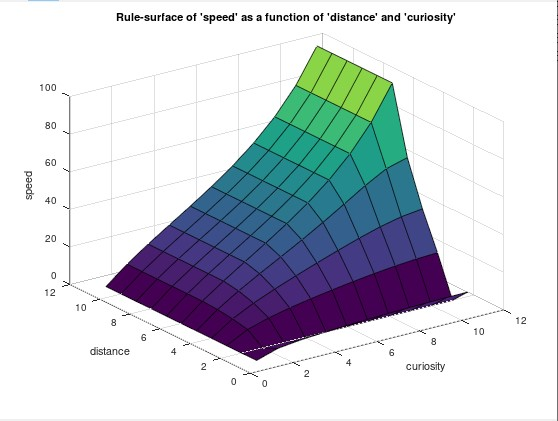
\includegraphics[width=1\textwidth]{images/rule_surface}
	\caption{Rule Surface}
	\label{fig:combined}
\end{figure}

Examining these rules separately we see how the ``speed'' value changes: figure \ref{fig:curiosity} in case of curiosity and figure \ref{fig:distance} for distance.

\pagebreak

\begin{figure}[!h]
	\centering
	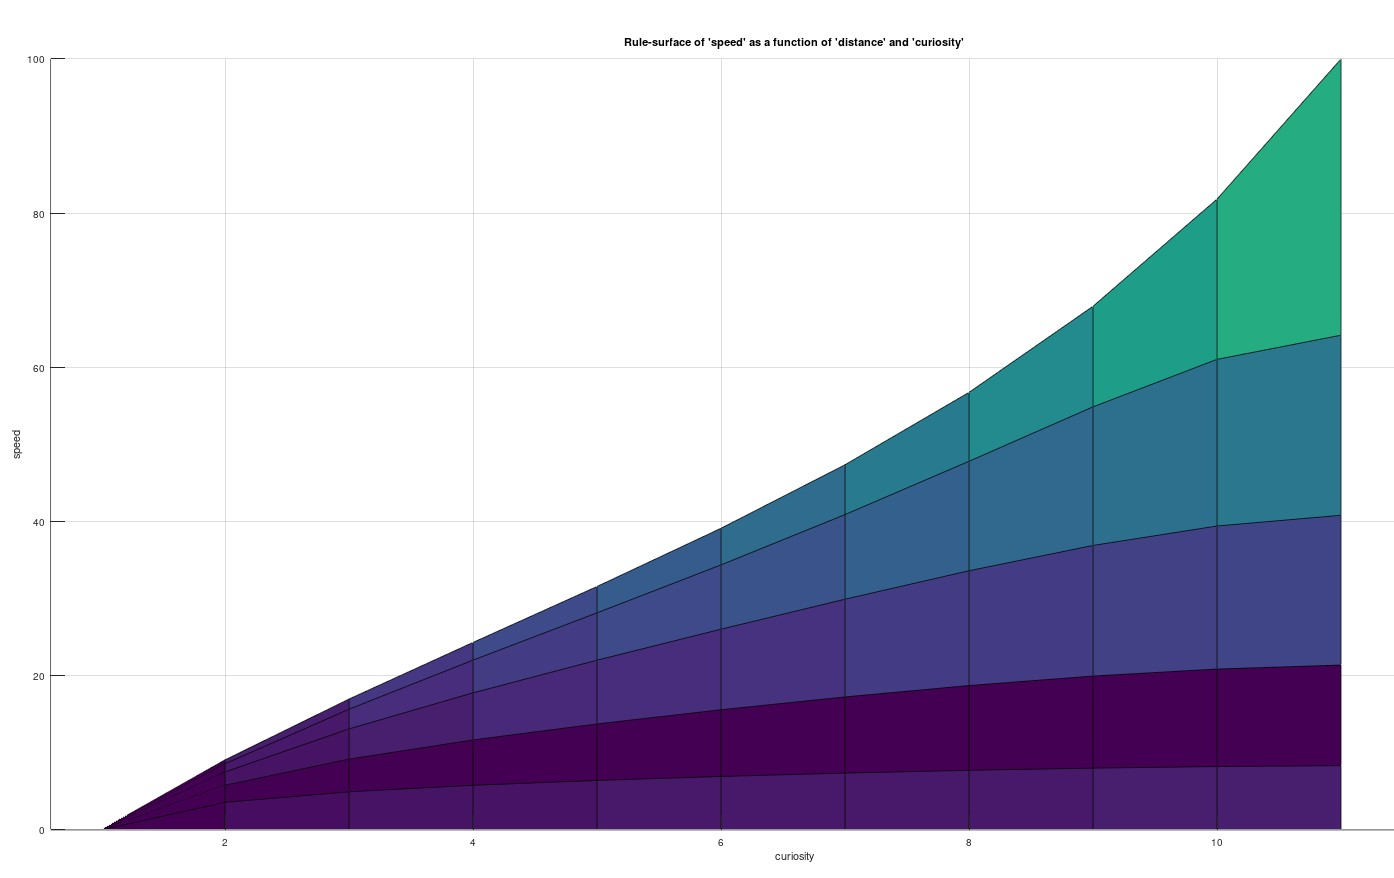
\includegraphics[width=1\textwidth]{images/curiosity}
	\caption{Curiosity}
	\label{fig:curiosity}
\end{figure}

\begin{figure}[!h]
	\centering
	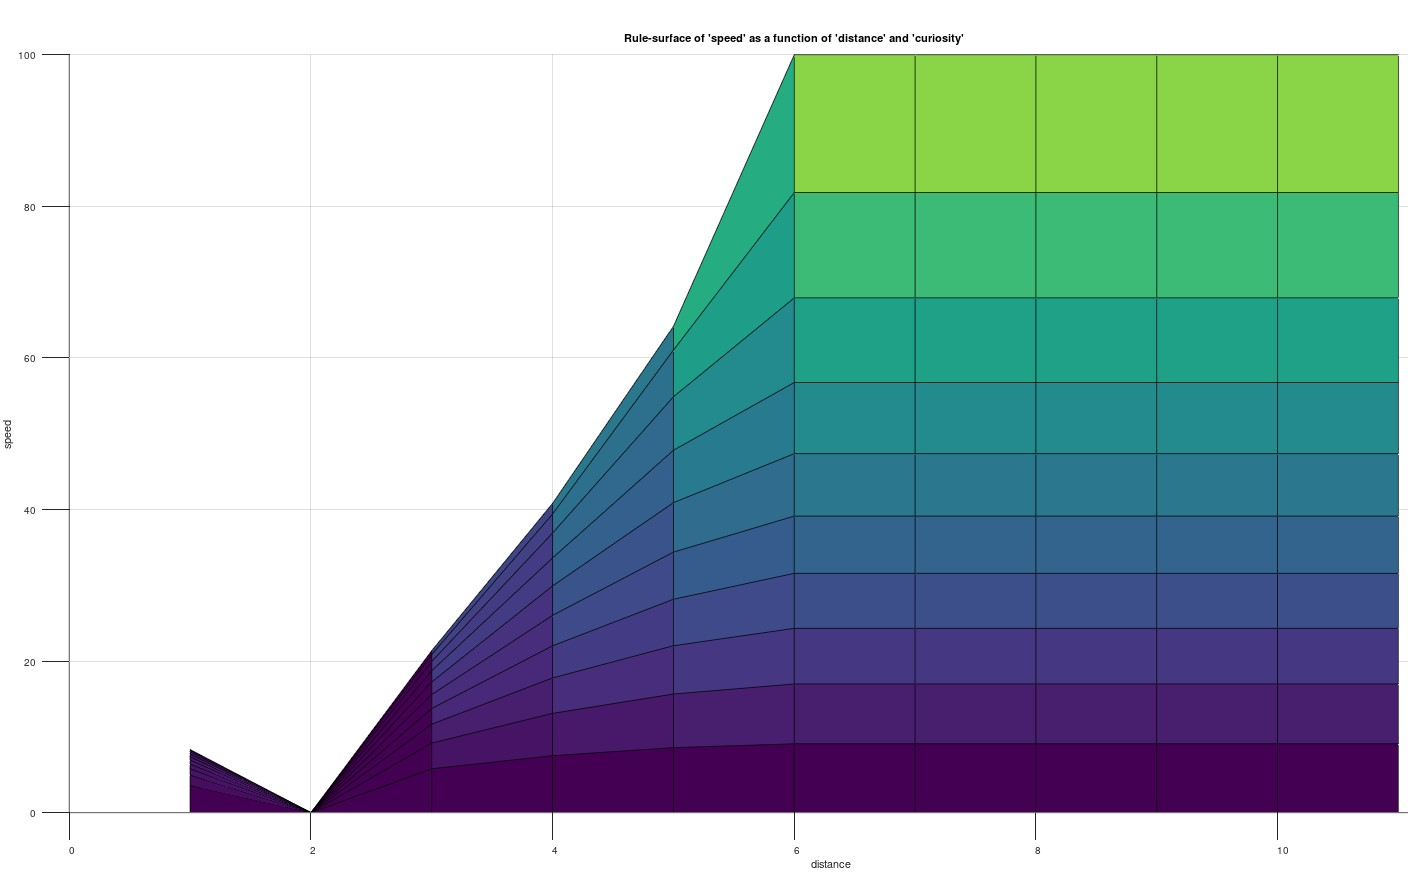
\includegraphics[width=1\textwidth]{images/distance}
	\caption{Distance}
	\label{fig:distance}
\end{figure}
